\documentclass[letterpaper,11pt]{article}
\usepackage{science}
\usepackage[utf8]{inputenc}
\usepackage{mathtools}
\usepackage{subcaption}
\usepackage{tikz}
\usepackage{pgf}
\usepackage{pgfplots}
\usepackage{circuitikz}
\usepackage{tabularx}
\usepackage{array}
\usepackage{booktabs} 
\usepackage{colortbl} 
\usepackage{xfrac}
\usepackage{gensymb}
\usepackage{chemformula}

\usetikzlibrary{calc}

\title{\textbf{Ottica:} esperienza 5}
\author{Canteri Marco, Biasi Lorenzo, Damiani Emily}
\date{\today}

\begin{document}
\maketitle

\begin{abstract}
\hspace{-1.9em}
In questa esperienza abbiamo verificato la legge di Beer, che spiega come cambia l'intensità del raggio emergente rispetto a quello incidente quando questo passa attraverso un materiale. Nell'esperimento in questione è stata utilizzata una soluzione di solfato di rame (\ch{CuSO_4}), la relazione è stata verificata per variazioni di concentrazione della soluzione e per variazioni della lunghezza del cammino della luce.
\end{abstract}

\begin{body}
\section{Procedimento}
La legge da verificare sperimentalmente è la seguente: 
\begin{equation}
I_m = A \cdot e^{-\alpha (C) L}
\end{equation}
dove $I_m$ indica l'intensità del raggio emergente, mentre $\alpha$ una costante che è funzione della concentrazione della soluzione e $L$ la lunghezza del cammino percorso dalla luce nella soluzione. \\
Per il primo set di misure l'apparato sperimentale è stato montato come segue. Il laser punta verso una cuvetta con lunghezza di base $L = 10.4 \,\text{mm}$ contenente della soluzione di \ch{CuSO_4}, mentre il raggio uscente viene ricevuto dal foto detector che ne misura l'intensità $I_m$. Per verificare la legge ci siamo serviti di due laser a luce rossa e arancione. Inoltre, per ogni laser abbiamo preparato $6$ soluzioni alle seguenti concentrazioni: 
\begin{itemize}
\item $0.8 \,\text{M}$
\item $0.6 \,\text{M}$
\item $0.5 \,\text{M}$
\item $0.25 \,\text{M}$
\item $0.125 \,\text{M}$
\item $0.062 \,\text{M} $ 
\end{itemize}
Le provette alle diverse concentrazioni sono state preparate a partire da un'unica soluzione di solfato di rame 1 M, diluita poi con acqua. \\
Le misure col fotodetector sono state eseguite il più velocemente possibile, in modo che non si verificasse un cambio nell'intensità del raggio incidente, che avrebbe influenzato le misure di intensità $I_m$. Oltre alle 6 misure a concentrazione diverse, abbiamo preso anche le misure di provette contenente la sostanza $1M$ e sola acqua.\\
Le misure per piccoli cambiamenti di lunghezza sono state effettuate nelle stesse condizioni. Stavolta si è mantenuta fissa la concentrazione, variando invece le lunghezze dei contenitori della soluzione.\\
Durante l'esperimento si è registrata il valore dell'intensità di fondo in modo da correggere un eventuale errore di offset.

\section{Analisi Dati}

Dividiamo la discussione sui set di misure in due parti, relative alle due modalità differenti per verificare la legge di Beer. 
\subsection{Misure in funzione della concentrazione}

\begin{figurehere}
\centering
\scalebox{1}{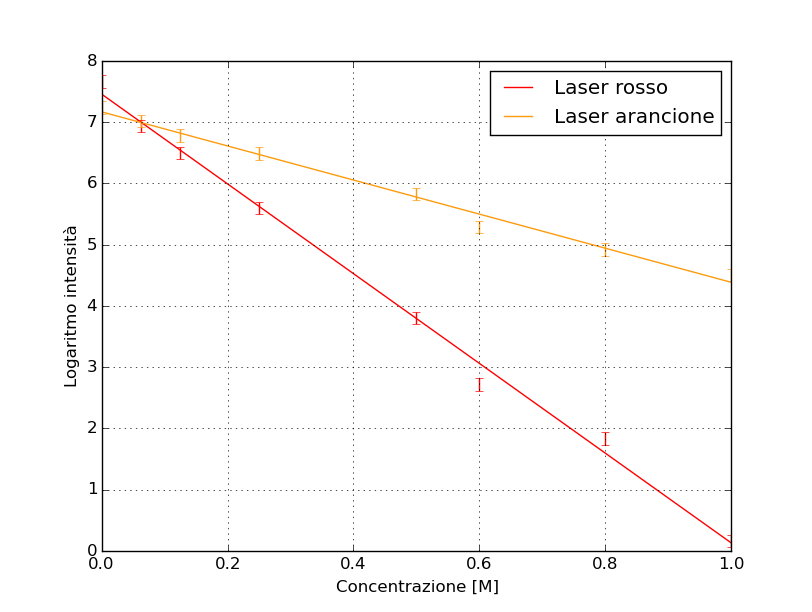
\includegraphics[width=.5\textwidth]{prima.png}}
\caption{Regressione lineare}
\end{figurehere}\leavevmode
\\
La prima parte dell'analisi riguarda la verifica della legge di beer in funzione della concentrazione a lunghezza L fissata. La legge di Beer ha forma esponenziale, ma può essere facilmente ridotta a una relazione lineare: 
\begin{equation}
\ln(I_m) = \ln(A) - \alpha(C) L
\end{equation}
La dipendenza diretta con la concentrazione è messa in evidenza riscrivendo la costanza $\alpha$ come il prodotto della costante caratteristica della soluzione $K$ e $C$.
\begin{equation}
\label{reg}
\ln(I_m) = \ln(A) - KLC
\end{equation}
Avendo a disposizione il set di dati in funzione della concentrazione, si procede con la regressione lineare della relazione precedente e si estrae il valore del coefficiente $K$:\\

\begin{tablehere}
\centering
\begin{tabular}{c|c|c}
\toprule
Laser& K [$\text{Mm}^{-1}$ ]& $\chi^2$\\
\midrule
rosso &  $704.6\pm 0.1 $& 2.8 \\
arancione & $267.6\pm 0.1$  & 0.9 \\
\bottomrule
\end{tabular}
\caption{Valori ottenuti dalla regressione, $\chi^2$ normalizzato}
\end{tablehere}\leavevmode
\subsection{Misure in funzione della lunghezza}
\begin{figurehere}
\centering
\scalebox{1}{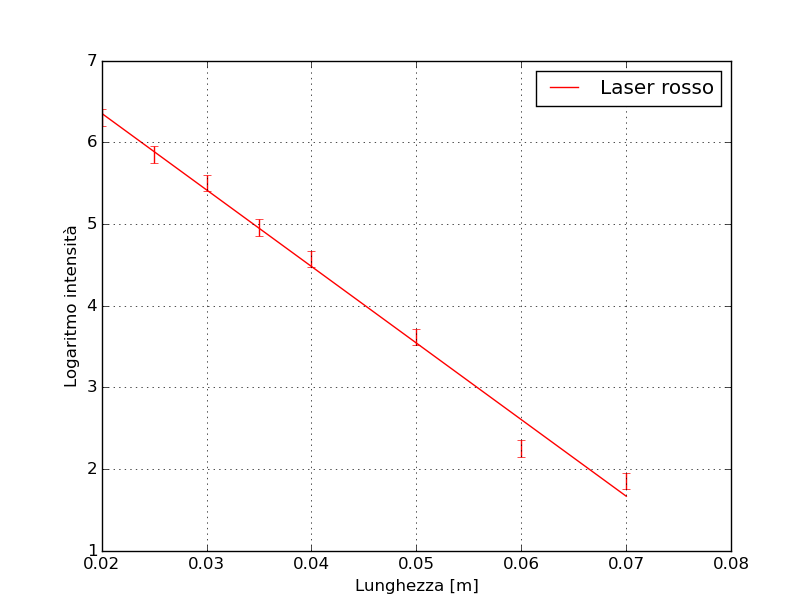
\includegraphics[width=.5\textwidth]{seconda.png}}
\caption{Regressione lineare}
\end{figurehere}\leavevmode
\\
L'equazione \eqref{reg} si può sfruttare anche per la regressione in funzione della lunghezza $L$, 
si ricava di nuovo il parametro $K$:
\[K = 750.4 \pm 2.1 \, \text{Mm}^{-1}\]
con $\chi^2$ normalizzato di 2.3.




\end{body}
\end{document}
